\documentclass[main.tex]{subfiles}
\begin{document}
\section{Neutron Tagging with the analog setup}

1 hour of measurements $4.3\cdot 10^{6}$ events were recorded by the analog setup. The immediate output is 4 tdc spectrums Giving the time differences for NE213 hits and the respective YAPs. qdc spectra, one for each yap, and two qdc spectra for the NE213 detector (one longgate and one shortgate).
\subsection{NE213 QDC spectrum}
The energy registered in the longgate QDC is shown in fig \ref{fig:qdc_a}. The 2.23 MeV Compton edges are visible near bin 1200 and the 4.4 MeV Compton edge is visible around bin 2900. Using the Knox method a linear fit has been made to the data.
\begin{figure}[ht!]
    \centering
        \includegraphics[width=\textwidth]{AnalogResults/Ecall.pdf}
        \caption{The pedestal along with the 2.23 and 4.44 MeV Compton edges have here been used to perform an energy calibration.}
    \label{fig:qdc_a}
\end{figure}

\newpage
\subsubsection{YAP QDC spectrum}
Write about scattered gammas that are both stop and start signals. Geometry dependent. Analog setup only records when there is a ToF coincidence, so scattered gammas end up dominating the yap qdc spectrum, which leads to the yap closest to the NE213 always having the largest gamma peak in the ToF spectrum. 

\newpage
\subsection{Pulse shape discrimination}
\subsubsection{Charge comparison method}
Since neutrons and gammas interact differently in the NE213 detector their signal has different shape and duration. This makes it possible to discriminate between neutrons and gammas.
\begin{figure}
    \centering
        \includegraphics[width=\textwidth]{AnalogResults/psd.pdf}
        \caption{Since a larger fraction of the neutrons energy deposition is located in the tail of their signals the upper band consists mainly of neutrons. The 2.23 and 4.44 MeV gamma edges can clearly be seen in the gamma band below.}
        \label{fig:hex_a}
\end{figure}
\newpage
\subsection{Time of Flight spectrum}
\begin{figure}[ht]
    \centering
        \includegraphics[width=\textwidth]{AnalogResults/tof.pdf}
        \caption{The time of flight spectrum.}
    \label{fig:A_TOF}
\end{figure}

\subsubsection{Pulse shape and ToF}
\begin{figure}[ht]
    \centering
        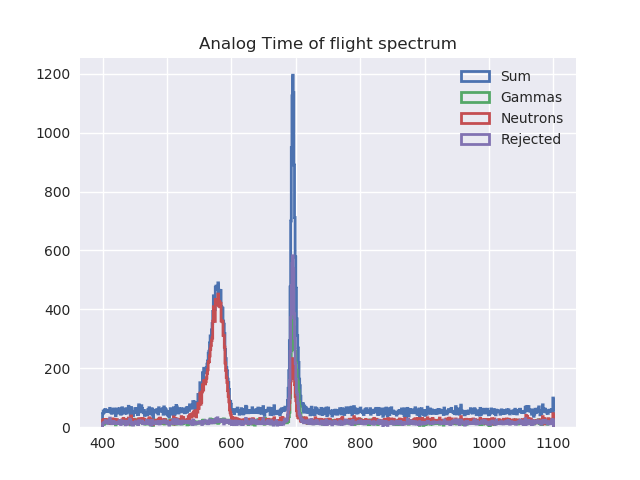
\includegraphics[width=\textwidth]{AnalogResults/tof_psd.pdf}
        \caption{Plotting the tail/total ratio against the time of flight shows that what we are separating with this parameter is indeed neutrons and gammas. There is however some overlap.}
    \label{fig:tof_ps_a} 
\end{figure}





\end{document}
